\documentclass[12pt]{article}
\usepackage{amsfonts}
\usepackage{amsmath}
\usepackage{bm}
\usepackage{bbm}
\usepackage{graphicx}
\usepackage{geometry}[margin=1in]


\title{Regionally Additive Models: Explainable-by-design models minimizing feature interactions}

\newcommand{\Rd}{\mathbb{R}^d}
\newcommand{\xb}{\mathbf{x}}
\newcommand{\xc}{\mathbf{x_c}}
\newcommand{\fxc}{f^{(\xc)}}
\newcommand{\fxs}{f^{(x_s)}}
\newcommand{\Xcal}{\mathcal{X}}
\newcommand{\Ycal}{\mathcal{Y}}
\newcommand{\when}[1]{\mathbbm{1}_{#1}}

\author{Vasilis Gkolemis}


\begin{document}
\maketitle

\begin{abstract}
Generalized Additive Models (GAMs) are a popular class of explainable-by-design models that are widely used in practice.
GAMs are based on the assumption that the effect of each feature on the target is independent of the values of the
other features, however, in cases where this assumption is violated they may lead to poor performance.
To address this limitation we propose Regionally Additive Models (RAMs), a novel class of explainable-by-design models,
that fits multiple GAMs to subregions of the feature space where interactions are minimized.
Our approach consists of two steps: first, we fit a black-box model and we identify the subregions where the black-box model is nearly locally additive,
i.e., where the effect of each feature on the target is independent of the values of the other features.
Secondly, we train a GAM specifically for each identified subregion.

We show that RAMs are more expressive than GAMs while they are still interpretable.

\end{abstract}

\section{Introduction}

To motivate about the use of RAMs, consider the black-box function
\(f(\xb) = 8x_2\when{x_1 > 0}\when{x_3=0}\) with \(x_1, x_2 \sim \mathcal{U}(-1,1)\) and \(x_3 \sim Bernoulli(0,1)\).
The black-box function $f$ involves an interaction term between the three features.
In principle, such interactions cannot be captured by a GAM which is a linear combination of univariate functions.
However, the black-box if we split the input space in two regions we observe that $f$ is locally additive
in each one, i.e.,

\begin{equation}
    f(\xb) = \begin{cases} 8x_2 & \text{if } x_1 > 0 \text{ and } x_3 = 0 \\ 0 & \text{otherwise} \end{cases}
\end{equation}
%
which makes it trivial to fit a separate GAMs in each subregion.

Correctly identifying the regions where the black-box function is locally additive is the key idea behind RAMs.
This can be handled


\begin{figure}[htbp]
    \centering
    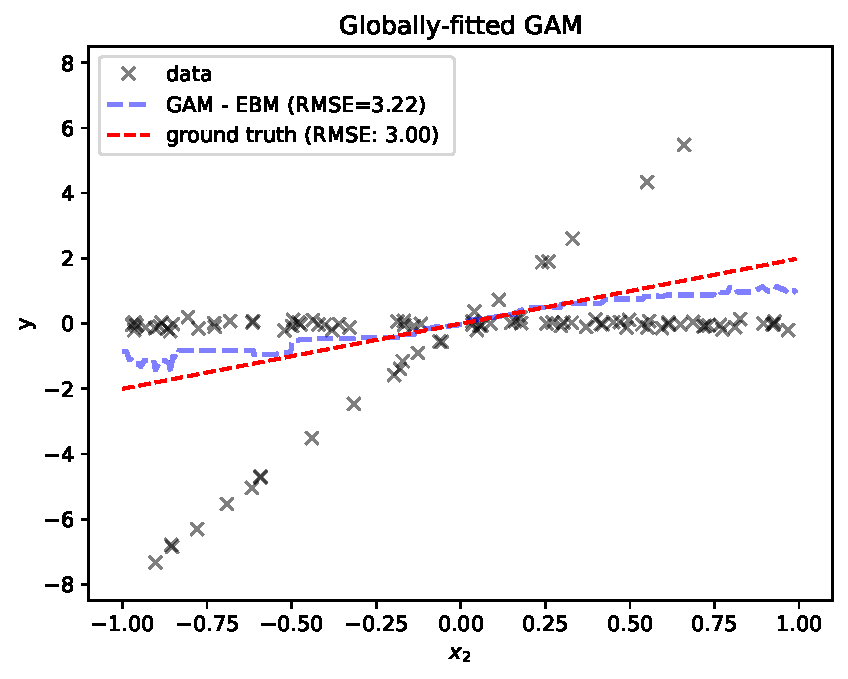
\includegraphics[width=0.32\textwidth]{figures/global_GAM.pdf}
    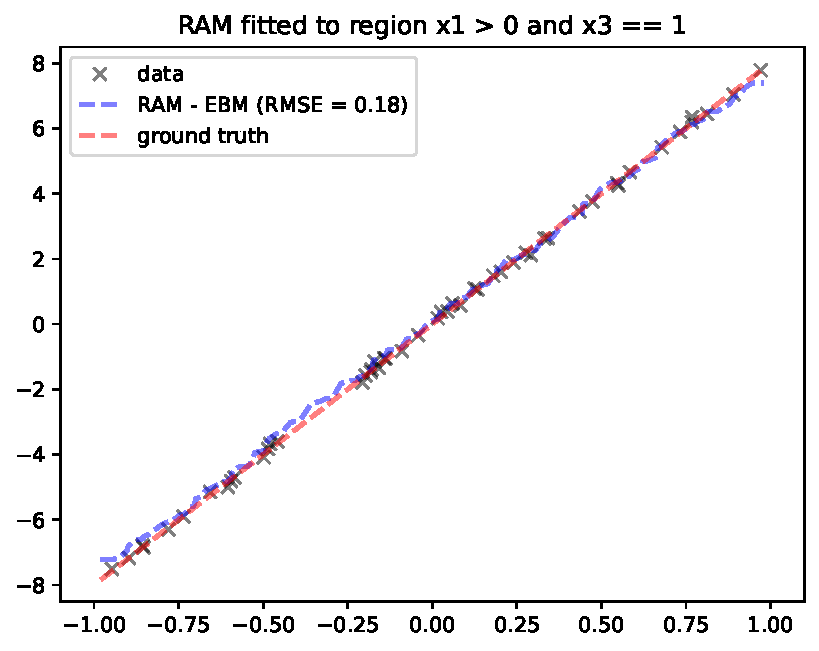
\includegraphics[width=0.32\textwidth]{figures/regional_gam_subreg_1.pdf}
    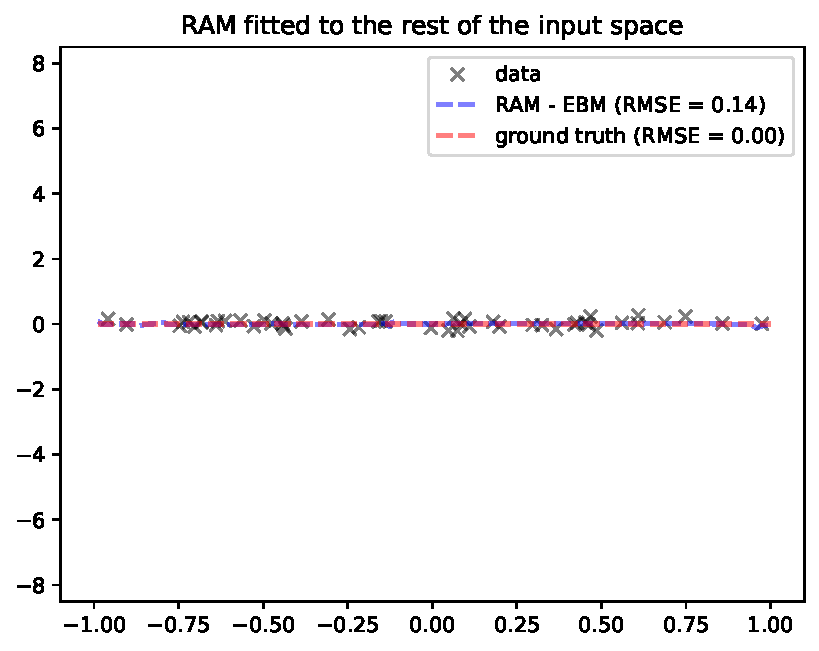
\includegraphics[width=0.32\textwidth]{figures/regional_gam_subreg_2.pdf}
    \caption{Caption}
\end{figure}

\section{Background}

Let \(\Xcal \in \Rd\) be the \(d\)-dimensional feature space, \(\Ycal\) the target space and \(f(\cdot) : \Xcal \rightarrow \Ycal\) the black-box function.  We use index \(s \in \{1, \ldots, d\}\) for the feature of interest and \(c = \{1, \ldots, d\} - s\) for the rest.
For convenience, we use \((x_s, \xc)\) to refer to \((x_1, \cdots , x_s, \cdots, x_D)\) and, equivalently, \((X_s, X_c)\) instead of \((X_1, \cdots , X_s, \cdots, X_D)\) when we refer to random variables.
The training set \(\mathcal{D} = \{(\xb^i, y^i)\}_{i=1}^N\) is sampled
i.i.d.\ from the distribution \(\mathbb{P}_{X,Y}\).  Finally,
\(f^{\mathtt{<method>}}(x_s)\) denotes how \(\mathtt{<method>}\)
defines the feature effect and \(\hat{f}^{\mathtt{<method>}}(x_s)\)
how it estimates it from the training set.

\section{RAM: Regionally Additive Models}




%Feature Effect (FE) methods explain the `black-box` function $f: \mathbb{R}^D \rightarrow \mathbb{R}$
%with a set of $1D$ mappings $f_s(x_s): \mathbb{R} \rightarrow \mathbb{R}$,
%each one being the effect of the $s$-th feature on the output.
%For example, [running example]..
%
%In this study, we propose interpreting FE as global surrogate models,
%i.e., as algorithms that take as input (a) the black-box function $f$ and (b) the training set $\mathcal{D}$ and
%they output a generalized additive model $f_{\mathtt{FE}}(\xb) = c + \sum_{s=1}^D f_s(x_s)$.
%Using this perspective, we will discuss the different approaches for defining the feature effect and we will
%propose a quantitative framework for evaluating them.
%
%\subsection{Approaches}
%
%At Table~\ref{tab:fe-methods}, we present the most used feature effect methods, namely,
%(a) the Partial Dependence Plot (PDP),
%(b) the derivative of the PDP (d-PDP)
%(c) the M-Plots and
%(d) the Accumulated Local Effects (ALE) plots.
%
%\begin{table}[htbp]
%    \centering
%    \caption{Table Caption}
%    \label{tab:fe-methods}
%    \begin{tabular}{c|c|c}
%      \hline
%      \textbf{Name} & \textbf{Definition} \(f(x_s)\) & \textbf{Approximation} \(\hat{f}(x_s)\)\\
%      \hline
%      \textbf{PDP} & $\mathbb{E}_{X_c}[f(x_s,X_c)]$ & $\frac{1}{N} \sum f(x_s,x_c^{(i)})$ \\
%      \hline
%      \textbf{d-PDP} & $\mathbb{E}_{X_c}[ \frac{\partial f(x_s,X_c)}{\partial x_s}]$ & $\frac{1}{N} \sum \frac{\partial f(x_s,x_c^{(i)})}{\partial x_s}$ \\
%      \hline
%      \textbf{M-Plot} & $\mathbb{E}_{X_c|x_s}[f(x_s,X_c)]$ & $\frac{1}{N} \sum_{i: x_s^{i} \in B(x_s)} f(x_s,x_c^{(i)})$ \\
%      \hline
%      \textbf{ALE} & \(\int_{x_{s,\min}}^{x_s} \mathbb{E}_{X_c|X_s=z}\left [f^s (z, X_c)\right ] \partial z\) & $\Delta x \sum_{k=1}^{k_x} \frac{1}{|\mathcal{S}_k|} \sum_{i:\mathbf{x}^{(i)} \in
%                                                                                                                \mathcal{S}_k} f^s(\mathbf{x}^i)$ \\
%      \hline
%    \end{tabular}
%\end{table}
%
%Global surrogate methods are evaluated based on their fidelity, i.e.,
%how well they can replicate the underlying black-box function.
%
%    \section{Interaction Index}
%    \subsection{Approaches}
%    \section{Regional Effects}
%    \subsection{Approaches}
%
%    \section{A unified evaluation framework}
%
%    \subsection{Idea 1}
%
%    We may split every $f: \mathbb{R}^D \rightarrow \mathbb{R}$ into
%    a model without interaction between $\xc$ and $x_s$,
%    i.e., $f_{ni}(\xb) = \fxs(x_s) +  \fxc(\xc)$,
%    and the interaction term $\kappa(\xc, x_s)$:
%
%    \[
%      f(\xb) = \underbrace{\fxs(x_s) +  \fxc(\xc)}_{f_{ni}(\xb)} + \kappa(\xc, x_s)
%    \]
%
%    A simple approach is defining \(f\) to be a Neural Network and \(f_{ni}\) a Neural Additive Model without interaction
%    between \(x_s\) and \(\xc\). Then \(\kappa(\xc, x_s) = f(\xb) - f_{ni}(\xb)\) and we quantify the importance of \(\kappa\) as \(\mathbb{E}_{X_c, X_s} \left [ |\kappa(X_c, X_s)| \right ] \approx \sqrt{\frac{1}{N} \sum_i \kappa^2(\xc, x_s)} \).
%
%    \subsection{Idea 2}

\section{Synthetic Examples}

\section{Real-World Datasets}


\end{document}
